\documentclass[aspectratio=169]{./latex_main/tntbeamer}  % you can pass all options of the beamer class, e.g., 'handout' or 'aspectratio=43'
\usepackage{dsfont}
\usepackage{bm}
\usepackage[english]{babel}
\usepackage[T1]{fontenc}
%\usepackage[utf8]{inputenc}
\usepackage{graphicx}
\graphicspath{ {./figures/} }
\usepackage{algorithm}
\usepackage[ruled,vlined,algo2e,linesnumbered]{algorithm2e}
\usepackage{hyperref}
\usepackage{booktabs}
\usepackage{mathtools}

\usepackage{amsmath,amssymb}
\usepackage{latexsym}

\DeclareMathOperator*{\argmax}{arg\,max}
\DeclareMathOperator*{\argmin}{arg\,min}

\usepackage{pgfplots}
\pgfplotsset{compat=1.16}
\usepackage{tikz}
\usetikzlibrary{trees} 
\usetikzlibrary{shapes.geometric}
\usetikzlibrary{positioning,shapes,shadows,arrows,calc,mindmap}
\usetikzlibrary{positioning,fadings,through}
\usetikzlibrary{decorations.pathreplacing}
\usetikzlibrary{intersections}
\pgfdeclarelayer{background}
\pgfdeclarelayer{foreground}
\pgfsetlayers{background,main,foreground}
\tikzstyle{activity}=[rectangle, draw=black, rounded corners, text centered, text width=8em]
\tikzstyle{data}=[rectangle, draw=black, text centered, text width=8em]
\tikzstyle{myarrow}=[->, thick, draw=black]

% Define the layers to draw the diagram
\pgfdeclarelayer{background}
\pgfdeclarelayer{foreground}
\pgfsetlayers{background,main,foreground}

\newcommand{\comment}[1]{
	\noindent
	%\vspace{0.25cm}
	{\color{red}{\textbf{TODO:} #1}}
	%\vspace{0.25cm}
}
\newcommand{\notefh}[1]{\textcolor{red}{\textbf{FH:} #1}}
\renewcommand{\comment}[1]{}
\newcommand{\hide}[1]{}
\newcommand{\cemph}[2]{\emph{\textcolor{#1}{#2}}}

%\newcommand{\lit}[1]{{\footnotesize\color{black!60}[#1]}}

%\newcommand{\litw}[1]{{\footnotesize\color{blue!20}[#1]}}


\newcommand{\myframe}[2]{\begin{frame}[c]{#1}#2\end{frame}}
\newcommand{\myframetop}[2]{\begin{frame}{#1}#2\end{frame}}
\newcommand{\myit}[1]{\begin{itemize}#1\end{itemize}}
\newcommand{\myblock}[2]{\begin{block}{#1}#2\end{block}}


\newcommand{\votepurple}[1]{\textcolor{Purple}{$\bigstar$}}
\newcommand{\voteyellow}[1]{\textcolor{Goldenrod}{$\bigstar$}}
\newcommand{\voteblue}[1]{\textcolor{RoyalBlue}{$\bigstar$}}
\newcommand{\votepink}[1]{\textcolor{Pink}{$\bigstar$}}

\newcommand{\diff}{\mathop{}\!\mathrm{d}}
\newcommand{\refstyle}[1]{{\small{\textcolor{gray}{#1}}}}
\newcommand{\hands}[0]{\includegraphics[height=1.5em]{images/hands}}
\newcommand{\transpose}[0]{{\textrm{\tiny{\sf{T}}}}}
\newcommand{\norm}{{\mathcal{N}}}
\newcommand{\cutoff}[0]{\kappa}
\newcommand{\instD}[0]{\dataset}
\newcommand{\insts}[0]{\mathcal{I}}
\newcommand{\inst}[0]{i}
\newcommand{\instI}[1]{i^{(#1)}}

% Iteration specific instance of variable/function/anything
% Introduced in the BO section, but moved up here to make it available within other macros
\newcommand{\iter}[2][\bocount]{{#2}^{(#1)}}

%--------HPO parameter macros-----------

% Parameter Configuration Space
\newcommand{\pcs}[0]{\pmb{\Lambda}}

% ???
\newcommand{\bx}[0]{\conf}

% Parameter Configuration
\newcommand{\conf}[0]{\pmb{\lambda}}

% Final Configuration
\newcommand{\finconf}[0]{\pmb{\hat{\lambda}}}

% Configuration corresponding to a given iteration -- better use \iter!
\newcommand{\confI}[1]{{\conf}^{(#1)}}

% Default Configuration
\newcommand{\defconf}[0]{{\conf}_{\text{def}}}

% Incumbent Configuration
\newcommand{\incumbent}[1][\bocount]{\iter[#1]{\finconf}}

% Optimal Configuration
\newcommand{\optconf}[0]{{\conf}^*}

% Configuration Space
\newcommand{\confs}[0]{\pcs}

%----------------------------------------

%\newcommand{\vlambda}[0]{\bm{\lambda}}
%\newcommand{\vLambda}[0]{\bm{\Lambda}}
\newcommand{\dataset}[0]{\mathcal{D}}
\newcommand{\datasets}[0]{\mathbf{D}}
\newcommand{\loss}[0]{L}
\newcommand{\risk}{\mathcal{R}}
\newcommand{\riske}{\mathcal{R}_{\text{emp}}}
\newcommand{\cost}[0]{c}
\newcommand{\costI}[1]{c^{(#1)}}

% Gaussian Process
\newcommand{\gp}{\mathcal{G}}
% Family of Objective Functions
\newcommand{\objF}{F}

%---------------BO Macros------------------

% BO loop counter
\newcommand{\bocount}{t}
% BO loop counter max, the counter runs from 1 to this value
\newcommand{\bobudget}{T}
% BO loop observation
\newcommand{\obs}[1][\conf]{\cost({#1})}
% BO loop observation space
\newcommand{\obsspace}{\mathcal{Y}}
% BO loop next observation
\newcommand{\bonextobs}{\obs[\iter{\conf}]}
% Acquisition Function, no args
\newcommand{\acq}{u}
% Standard Normal PDF
\newcommand{\pdf}{\phi}
% Standard Normal CDF
\newcommand{\cdf}{\Phi}
% Mean
\newcommand{\mean}{\mu}
% Standard Deviation
\newcommand{\stddev}{\sigma}
% Variance
\newcommand{\variance}{\sigma^2}
% Noise
\newcommand{\noise}{\nu}
% BO loop next selected sample
\newcommand{\bonextsample}{\confI{\bocount}}

% Single hyperparameter
\newcommand{\hyperparam}{\lambda}

% Single hyperparameter within a hyperparameter configuration
\newcommand{\hyperparami}[1][i]{{\hyperparam}_#1}

% Full definition of final configuration
\newcommand{\finconffull}{\incumbent[\bobudget]}

% Dataset
\newcommand{\datasetHPO}{{\dataset}_{HPO}}

% Dataset definition
\newcommand{\datasetHPOdef}{{\langle \bonextsample,\,\bonextobs \rangle}_{\bocount=1}^{\bobudget}}

% Double Display Fraction, forces large displays for everything in numerator and denominator
\newcommand\ddfrac[2]{\frac{\displaystyle #1}{\displaystyle #2}}

% Conditional Probability "Given That" Relation, source:https://tex.stackexchange.com/a/141685/205886
\newcommand\given[1][]{\:#1\vert\:}

% Expectation as a math operator
\DeclareMathOperator*{\E}{\mathbb{E}}

% Citation 
\newcommand{\source}[1]{
    \begin{flushright}
    	Source: \lit{#1}
    \end{flushright}
}
%-------------------------------------------

%Real numbers set
\newcommand{\realnum}{\mathbb{R}}
%Configuration space - do not use
%\newcommand{\configspace}{\Theta}
%Instances - do not use
%\newcommand{\instances}{\mathcal{I}}
%Expected value
\newcommand{\expectation}{\mathbb{E}}
%Kernel
\newcommand{\kernel}{\kappa}
%Constraint function
\newcommand{\constraintf}{c}
%Normal distribution
\newcommand{\normaldist}{\mathcal{N}}

% \renewcommand{\vec}[1]{\mathbf{#1}}
\newcommand{\hist}[0]{\dataset_{\text{Hist}}}
\newcommand{\param}[0]{p}
\newcommand{\algo}[0]{\mathcal{A}}
\newcommand{\algos}[0]{\mathbf{A}}
%\newcommand{\nn}[0]{N}
\newcommand{\feats}[0]{\mathcal{X}_{\text{meta}}}
\newcommand{\feat}[0]{\x_{\text{meta}}}
%\newcommand{\cluster}[0]{\vec{h}}
%\newcommand{\clusters}[0]{\vec{H}}
\newcommand{\perf}[0]{\mathbb{R}}
%\newcommand{\surro}[0]{\mathcal{S}}
\newcommand{\surro}[0]{\hat{\cost}}
\newcommand{\func}[0]{f}
\newcommand{\epm}[0]{\surro}
\newcommand{\portfolio}[0]{\mathbf{P}}
\newcommand{\schedule}[0]{\mathcal{S}}

% Machine Learning
\newcommand{\mdata}[0]{\dataset_{\text{meta}}}
\newcommand{\datasettrain}[0]{\dataset_{\text{train}}}
\newcommand{\datasetval}[0]{\dataset_{\text{val}}}
\newcommand{\datasettest}[0]{\dataset_{\text{test}}}
\newcommand{\x}[0]{\mathbf{x}}
\newcommand{\y}[0]{y}
\newcommand{\xI}[1]{\mathbf{x}^{(#1)}}
\newcommand{\yI}[1]{y^{(#1)}}
\newcommand{\fx}{f(\mathbf{x})}  % f(x), continuous prediction function
\newcommand{\Hspace}{\mathcal{H}} % hypothesis space where f is from
\newcommand{\fh}{\hat{f}}       % f hat, estimated prediction function

% Deep Learning
\newcommand{\weights}[0]{\theta}
\newcommand{\metaweights}[0]{\phi}


% reinforcement learning
\newcommand{\policies}[0]{\mathbf{\Pi}}
\newcommand{\policy}[0]{\pi}
\newcommand{\actionRL}[0]{a}
\newcommand{\stateRL}[0]{s}
\newcommand{\statesRL}[0]{\mathcal{S}}
\newcommand{\rewardRL}[0]{r}
\newcommand{\rewardfuncRL}[0]{\mathcal{R}}

%\RestyleAlgo{algoruled}
%\DontPrintSemicolon
%\LinesNumbered
%\SetAlgoVlined
%\SetFuncSty{textsc}

%\SetKwInOut{Input}{Input}
%\SetKwInOut{Output}{Output}
%\SetKw{Return}{return}

%\newcommand{\changed}[1]{{\color{red}#1}}

%\newcommand{\citeN}[1]{\citeauthor{#1}~(\citeyear{#1})}

\renewcommand{\vec}[1]{\mathbf{#1}}
%\DeclareMathOperator*{\argmin}{arg\,min}
%\DeclareMathOperator*{\argmax}{arg\,max}

%\newcommand{\aqme}{\textit{AQME}}
%\newcommand{\aslib}{\textit{ASlib}}
%\newcommand{\llama}{\textit{LLAMA}}
%\newcommand{\satzilla}{\textit{SATzilla}}
%\newcommand{\satzillaY}[1]{\textit{SATzilla'{#1}}}
%\newcommand{\snnap}{\textit{SNNAP}}
%\newcommand{\claspfolioTwo}{\textit{claspfolio~2}}
%\newcommand{\flexfolio}{\textit{FlexFolio}}
%\newcommand{\claspfolioOne}{\textit{claspfolio~1}}
%\newcommand{\isac}{\textit{ISAC}}
%\newcommand{\eisac}{\textit{EISAC}}
%\newcommand{\sss}{\textit{3S}}
%\newcommand{\sunny}{\textit{Sunny}}
%\newcommand{\ssspar}{\textit{3Spar}}
%\newcommand{\cshc}{\textit{CSHC}}
%\newcommand{\cshcpar}{\textit{CSHCpar}}
%\newcommand{\measp}{\textit{ME-ASP}}
%\newcommand{\aspeed}{\textit{aspeed}}
%\newcommand{\autofolio}{\textit{AutoFolio}}
%\newcommand{\cedalion}{\textit{Cedalion}}
\newcommand{\fanova}{\textit{fANOVA}}
\newcommand{\sbs}{\textit{SB}}
\newcommand{\oracle}{\textit{VBS}}

% like approaches
\newcommand{\claspfoliolike}[1]{\texttt{claspfolio-#1-like}}
\newcommand{\satzillalike}[1]{\texttt{SATzilla'#1-like}}
\newcommand{\isaclike}{\texttt{ISAC-like}}
\newcommand{\ssslike}{\texttt{3S-like}}
\newcommand{\measplike}{\texttt{ME-ASP-like}}

\newcommand{\irace}{\textit{I/F-race}}
\newcommand{\gga}{\textit{GGA}}
\newcommand{\smac}{\textit{SMAC}}
\newcommand{\paramils}{\textit{ParamILS}}
\newcommand{\spearmint}{\textit{Spearmint}}
\newcommand{\tpe}{\textit{TPE}}


\usepackage{pifont}
\newcommand{\itarrow}{\mbox{\Pisymbol{pzd}{229}}}
\newcommand{\ithook}{\mbox{\Pisymbol{pzd}{52}}}
\newcommand{\itcross}{\mbox{\Pisymbol{pzd}{56}}}
\newcommand{\ithand}{\mbox{\raisebox{-1pt}{\Pisymbol{pzd}{43}}}}

%\DeclareMathOperator*{\argmax}{arg\,max}

\newcommand{\ie}{{\it{}i.e.\/}}
\newcommand{\eg}{{\it{}e.g.\/}}
\newcommand{\cf}{{\it{}cf.\/}}
\newcommand{\wrt}{\mbox{w.r.t.} }
\newcommand{\vs}{{\it{}vs\/}}
\newcommand{\vsp}{{\it{}vs\/}}
\newcommand{\etc}{{\copyedit{etc.}}}
\newcommand{\etal}{{\it{}et al.\/}}

\newcommand{\pscProc}{{\bf procedure}}
\newcommand{\pscBegin}{{\bf begin}}
\newcommand{\pscEnd}{{\bf end}}
\newcommand{\pscEndIf}{{\bf endif}}
\newcommand{\pscFor}{{\bf for}}
\newcommand{\pscEach}{{\bf each}}
\newcommand{\pscThen}{{\bf then}}
\newcommand{\pscElse}{{\bf else}}
\newcommand{\pscWhile}{{\bf while}}
\newcommand{\pscIf}{{\bf if}}
\newcommand{\pscRepeat}{{\bf repeat}}
\newcommand{\pscUntil}{{\bf until}}
\newcommand{\pscWithProb}{{\bf with probability}}
\newcommand{\pscOtherwise}{{\bf otherwise}}
\newcommand{\pscDo}{{\bf do}}
\newcommand{\pscTo}{{\bf to}}
\newcommand{\pscOr}{{\bf or}}
\newcommand{\pscAnd}{{\bf and}}
\newcommand{\pscNot}{{\bf not}}
\newcommand{\pscFalse}{{\bf false}}
\newcommand{\pscEachElOf}{{\bf each element of}}
\newcommand{\pscReturn}{{\bf return}}

%\newcommand{\param}[1]{{\sl{}#1}}
\newcommand{\var}[1]{{\it{}#1}}
\newcommand{\cond}[1]{{\sf{}#1}}
%\newcommand{\state}[1]{{\sf{}#1}}
%\newcommand{\func}[1]{{\sl{}#1}}
\newcommand{\set}[1]{{\Bbb #1}}
%\newcommand{\inst}[1]{{\tt{}#1}}
\newcommand{\myurl}[1]{{\small\sf #1}}

\newcommand{\Nats}{{\Bbb N}}
\newcommand{\Reals}{{\Bbb R}}
\newcommand{\extset}[2]{\{#1 \; | \; #2\}}

\newcommand{\vbar}{$\,\;|$\hspace*{-1em}\raisebox{-0.3mm}{$\,\;\;|$}}
\newcommand{\vendbar}{\raisebox{+0.4mm}{$\,\;|$}}
\newcommand{\vend}{$\,\:\lfloor$}


\newcommand{\goleft}[2][.7]{\parbox[t]{#1\linewidth}{\strut\raggedright #2\strut}}
\newcommand{\rightimage}[2][.3]{\mbox{}\hfill\raisebox{1em-\height}[0pt][0pt]{\includegraphics[width=#1\linewidth]{#2}}\vspace*{-\baselineskip}}


% Requires XeLaTeX or LuaLaTeX
\usepackage{unicode-math}

\usepackage{fontspec}
%\setsansfont{Arial}
\setsansfont{RotisSansSerifStd}[ 
Path=./latex_main/fonts/,
Extension = .otf,
UprightFont = *-Regular,  % or *-Light
BoldFont = *-ExtraBold,  % or *-Bold
ItalicFont = *-Italic
]
\setmonofont{Cascadia}[
	Path=./latex_main/fonts/,
	Scale=0.8
]

% scale factor adapted; mathrm font added (Benjamin Spitschan @TNT, 2021-06-01)
%\setmathfont[Scale=1.05]{Libertinus Math}
%\setmathrm[Scale=1.05]{Libertinus Math}

% other available math fonts are (not exhaustive)
% Latin Modern Math
% XITS Math
% Libertinus Math
% Asana Math
% Fira Math
% TeX Gyre Pagella Math
% TeX Gyre Bonum Math
% TeX Gyre Schola Math
% TeX Gyre Termes Math

% Literature References
% #1 = Display Name
% #2 = Url (without \href)
\newcommand{\lit}[2]{\href{#2}{\footnotesize\color{black!60}[#1]}}

%%% Beamer Customization
%----------------------------------------------------------------------
% (Don't) Show sections in frame header. Options: 'sections', 'sections light', empty
\setbeamertemplate{headline}{empty}

% Add header logo for normal frames
\setheaderimage{
	% \includegraphics[height=\logoheight]{figures/TNT_darkv4.pdf}
	\includegraphics[height=\logoheight]{../latex_main/figures/luh_logo_rgb_0_80_155.pdf}
	% \includegraphics[height=\logoheight]{figures/logo_tntluh.pdf}
}

% Header logo for title page
\settitleheaderimage{
	% \includegraphics[height=\logoheight]{figures/TNT_darkv4.pdf}
	\includegraphics[height=\logoheight]{../latex_main/figures/luh_logo_rgb_0_80_155.pdf}
	% \includegraphics[height=\logoheight]{figures/logo_tntluh.pdf}
}

% Title page: tntdefault 
\setbeamertemplate{title page}[tntdefault]  % or luhstyle
% Add optional title image here
%\addtitlepageimagedefault{\includegraphics[width=0.65\textwidth]{figures/luh_default_presentation_title_image.jpg}}

% Title page: luhstyle
% \setbeamertemplate{title page}[luhstyle]
% % Add optional title image here
% \addtitlepageimage{\includegraphics[width=0.75\textwidth]{figures/luh_default_presentation_title_image.jpg}}

\author[Lindauer]{Marius Lindauer\\[1em]
	\includegraphics[height=\logoheight]{../latex_main/figures/luh_logo_rgb_0_80_155.pdf}\qquad
\includegraphics[height=\logoheight]{../latex_main/figures/TNT_darkv4}\qquad
\includegraphics[height=\logoheight]{../latex_main/figures/L3S.jpg}	}
\date{Winter Term 2021
}


%%% Custom Packages
%----------------------------------------------------------------------
% Create dummy content
\usepackage{blindtext}

% Adds a frame with the current page layout. Just call \layout inside of a frame.
\usepackage{layout}


\title[ML-RL: Big Picture]{Welcome to the RL Lecture}
\subtitle{Brief Motivation and Orga}
\graphicspath{w01_big_picture}

%\input{latex_main/main.tex}




\begin{document}
	
	\maketitle

%----------------------------------------------------------------------
%----------------------------------------------------------------------
\begin{frame}[c]{Question}
	
	\centering
	{
	\huge
	Why are you interested to learn more about reinforcement learning (RL)?
	}

	%\bigskip	\bigskip
	%$\to$ use the chat to answer!
	
\end{frame}
%-----------------------------------------------------------------------
%----------------------------------------------------------------------
\begin{frame}[c]{Machine Learning}

\centering
\textit{``Machine learning is the science of getting computers to act\\
 without being explicitly programmed.''}

\hfill by Andrew Ng

\end{frame}
%-----------------------------------------------------------------------
%----------------------------------------------------------------------
\begin{frame}[c]{Reinforcement Learning}
	
	\centering
	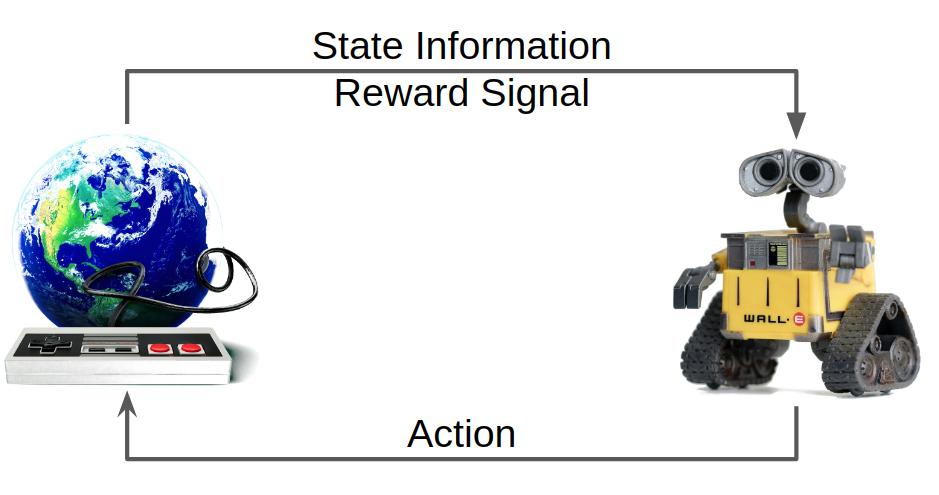
\includegraphics[width=0.55\textwidth]{images/rl_comic.png}\footnote{Image source: Morning Brew and Marius Haakestad on Unsplash}
	
	\bigskip
	
	\begin{itemize}
		\item Data: Self-acquired observations + rewards
		\item Task: Learn how to behave s.t. reward is maximized
		\item[$\leadsto$] Not a single decision, but a sequence of good decisions
	\end{itemize}	
	
	
\end{frame}
%-----------------------------------------------------------------------

%----------------------------------------------------------------------
\begin{frame}[c]{Goals of the Lecture}
	
	You will be able to \ldots
	\begin{enumerate}
		\item understand and explain the basic algorithms in RL
		\smallskip
		\item discuss the assumptions and limitations of RL and its algorithms
		\smallskip
		\item decide which RL algorithm to use on a given environments
		\smallskip
		\item do research on RL yourself
		\begin{itemize}
			\item perfect opportunity to do a master project or thesis with us afterwards
		\end{itemize}
	\end{enumerate}
	
\end{frame}
%-----------------------------------------------------------------------
%----------------------------------------------------------------------
\begin{frame}[c]{Course Overview (tentative)}
	
	\begin{enumerate}
		\item Big Picture (Introduction)
		\item MDP, Policy, Value Iteration
		\item Policy Evaluation
		\item Model Free Control
		\item Linear Function Approximation
		\item Deep RL
		\item Policy Gradient
		\item Exploration
		\item Meta-RL
		\item Reproducibility in RL
		\item Project
	\end{enumerate}
	
	\pause
	$\leadsto$ More an introduction into RL!
	
\end{frame}
%----------------------------------------------------------------------
%----------------------------------------------------------------------
\begin{frame}[c]{Course Format}
	
	\begin{itemize}
		\item Concepts over details
		\begin{itemize}
			\item we provide references and links to papers\\ s.t. you can read up details!
		\end{itemize}
		\smallskip
		\item Interactive lecture and exercise sessions
		\begin{itemize}
			\item short inputs ($\sim$10-20min) followed by Q\&A
			\item interactive quizzes in exercise sessions to reinforce your knowledge
			\item[$\leadsto$] The success of it depends on whether you are willing to talk to us! 
		\end{itemize}
		\smallskip
		\item (Mostly) Practical exercises
		\begin{itemize}
			\item implement it, use it and play with it!
		\end{itemize}
	\end{itemize}
	
\end{frame}
%----------------------------------------------------------------------
%----------------------------------------------------------------------
\begin{frame}[c]{Team}
	
	\begin{columns}[T]
		
		\column{0.3\textwidth}
		\centering
		\includegraphics[height=10em]{images/lindauer}
		
		Prof. Dr.\\ Marius Lindauer
		
		\column{0.3\textwidth}
		\centering
		\includegraphics[height=10em]{images/eimer}
		
		Theresa Eimer\\
		
		\column{0.3\textwidth}
		\centering
		\includegraphics[height=10em]{images/schubert}
		
		Frederik Schubert \\
		
		
	\end{columns}
	
	
\end{frame}
%----------------------------------------------------------------------
%----------------------------------------------------------------------
\begin{frame}[c]{Organization (Lectures)}
	
	\begin{itemize}
		\item Meeting each week Thursday at 2pm (s.t).
		\pause
		%\item I will try to limit the lecture to 90min, but since I would like to have an interactive lecture, let's be a bit flexible.
		%\pause
		\item Each week, the lecture is divided into small parts.
		\pause
		\item We will not record or stream the lecture
	\end{itemize}
	
\end{frame}
%-----------------------------------------------------------------------

%----------------------------------------------------------------------
\begin{frame}[c]{Organization (Exercises)}
	
	\begin{itemize}
		\item Every Wednesday at 3pm
		\begin{itemize}
			\item Regular attendance highly recommended!
			\item No recording
		\end{itemize}
		\pause
		\item Discussion of mini examples (e.g., Mars Robot)
		\pause
		\item Interactive Kahoot quiz
		\pause
		\item Feedback to exercise sheet
		\begin{itemize}
			\item You don't need to achieve any point threshold
			\item But you need to submit something every week
		\end{itemize}
	
	\end{itemize}
	
\end{frame}
%-----------------------------------------------------------------------
%----------------------------------------------------------------------
\begin{frame}[c]{Organization (Exercise Assignments)}
	
	\begin{itemize}
	\item Every week, a new exercise sheet
	\begin{itemize}
		\item exercise focus is one week behind the lecture topics
		\item Most exercises will be practical, i.e., you have to implement something
		\item Team work highly recommended, team size at most 3! 
		\pause
		\item Build upon GitHub classroom $\leadsto$ enables auto-grading
		\begin{itemize}
			\item There will be an invitation link each week on each exercise sheet.
			\item You will have to click on the link on exercise sheet one to be able to form groups.
			\item Submit solutions via git
		\end{itemize}
		\pause
		\item Up to \alert{$9$ bonus points} for final grade, i.e., 3 grading boosts.
		\begin{itemize}
		    \item To get a bonus point, your solution has to be at least correct by $80\%$
		\end{itemize}
		\pause
		\item If we catch anyone at obvious cheating (incl. plagiarism),\newline we will kick them out.
	\end{itemize}
	\pause
	\item \alert{If you need help or have questions, use the chat!}
	\end{itemize}
	
\end{frame}
%-----------------------------------------------------------------------
%----------------------------------------------------------------------
\begin{frame}[c]{You need help?}
	
Priority list:
	\begin{enumerate}
		\item Ask your friends and peers
		\item Use our chat system via Mattermost (see Stud.IP for invitation link)
		\begin{itemize}
		    \item[$\leadsto$] Channel ``2021 RL Lecture''
			\item You can also answer the questions of your peers! 
			\item We will only reply if we have the feeling that it is necessary.
		\end{itemize}
		\item If there are organizational questions, contact Theresa or Frederik directly (via Mattermost)
		\item Only as the very last option, contact me ;-)
	\end{enumerate}
	
\end{frame}
%-----------------------------------------------------------------------
\begin{frame}{AI Courses at LUH}
    
    \centering
    \includegraphics[width=0.6\textwidth]{images/ai_luh.PNG}

\end{frame}
%----------------------------------------------------------------------
\begin{frame}[c]{Requirements for Attending}
	
	\begin{itemize}
		\item Basics of \alert{AI} (mandatory)
		\begin{itemize}
			\item Search, planning, optimization \ldots, expectations, \ldots
		\end{itemize}
		\pause
		\item Basics of \alert{Machine Learning} (mandatory)
		\begin{itemize}
			\item Classification, regression, clustering, decision tree, training-test split, cross validation, pre-processing \ldots
			\item For example, ML lecture by Prof. Rosenhahn
			\item to catch up (if nec.):
			\url{https://www.coursera.org/learn/machine-learning} 
		\end{itemize}
		\pause
		\item Knowledge and hands-on exp. in \alert{Deep Learning} (PyTorch)\\ (mandatory)
		\begin{itemize}
			\item feed-forward network, recurrent network, convolutions, learning rates, regularization, \ldots 
			\item For example, DL lecture by Prof. Anand
			\item to catch up (if nec.): \url{https://course.fast.ai/}
		\end{itemize}
		\pause
		\item Experience in \alert{Python and git} (mandatory)
		\begin{itemize}
			\item nearly all exercises will require 
			that you implement something in~Python and submit the solution to a git repo
		\end{itemize}
	\end{itemize}
	\pause
	$\leadsto$ If you solved the self-assessment test, you should be ready.
	
\end{frame}
%-----------------------------------------------------------------------
%----------------------------------------------------------------------
\begin{frame}[c]{Final Grading}
	
	\begin{itemize}
		\item Implement a larger project (worth $1-2$ weeks full time)
		\begin{itemize}
			\item You can propose your own project idea!
			\begin{itemize}
				\item Hand-in a short summary of the idea (half a page) and we will provide feedback regarding feasibility
			\end{itemize}
			\item Teamwork (at most 3) again possible
			\begin{itemize}
				\item Larger team $\to$ larger scope of the project
			\end{itemize}
		\end{itemize}
		\item ``Exam''
		\begin{itemize}
			\item First $15$ minutes: Present your project idea and results in the 
			\begin{itemize}
				\item Of course, everyone will present the project on their own
			\end{itemize}
			\item Second 15min: We will ask further questions about your project and how it relates to stuff you learned in the lecture.
		\end{itemize}	
	%	\item You will have the choice between a virtual and on-site exam.
	\end{itemize}
	
\end{frame}
%----------------------------------------------------------------------
%----------------------------------------------------------------------
\begin{frame}[c,fragile]{Material}
	
	\begin{itemize}
		\item Slides: \url{https://github.com/automl-edu/RL_lecture}
		\item Additional Material:
		\begin{itemize}
    		\item To get a deep understanding of RL,\\ you should also read some papers 
    		\item RL book by Sutton and Barto: 
    		\url{https://www.andrew.cmu.edu/course/10-703/textbook/BartoSutton.pdf}
    		\item Video lectures -- click on it!
    		\begin{itemize}
    			\item \lit{Emma Brunskill (2019-20)}{https://www.youtube.com/watch?v=FgzM3zpZ55o&list=PLRQmQC3wIq9yxKVK1qc0r2nPuInn92LmK&index=1}
    			\item \lit{Sergey Levine (2020)}{https://www.youtube.com/playlist?list=PL_iWQOsE6TfURIIhCrlt-wj9ByIVpbfGc}
    			\item \lit{David Silver (2015)}{https://www.youtube.com/playlist?list=PLbWDNovNB5mqFBgq7i3MY6Ui4zudcvNFJ}
    			\item \lit{Robot Learning by Jan Peters (2021)}{https://learn.ki-campus.org/courses/moocrobot-tud2021}
		\end{itemize}
	\end{itemize}
	\end{itemize}
	
\end{frame}
%----------------------------------------------------------------------
%----------------------------------------------------------------------
\begin{frame}[c]{Opportunities and Risks}
	
	\vspace{-1em}
	RL is an advanced lecture and we present it for the second time
	
	\medskip
	\pause
	
	Opportunities:
	\begin{itemize}
		\item RL is a very hot topic these days
		\item We will start with the basics and go step by step to the more advanced (research) topics
		\item The course will provide a solid background\\ for doing a master project/thesis in our group 
	\end{itemize}
	
	\pause
	
	Challenges:
	\begin{itemize}
		\item The research on RL is very active and there is so much progress\newline $\leadsto$ impossible to catch up with state of the art with one course
		\item The origins of RL go back to robotics, control, theory on bandits and computer science $\leadsto$ different notations
		\item You will find some typos and issues in the slides\newline $\leadsto$ please tell us if you find something
	\end{itemize}
	
	\pause
	$\to$ Give us some feedback and we will improve the course!
	
	
\end{frame}
%-----------------------------------------------------------------------

\begin{frame}[c]{}
	
	\centering
	\huge
	Questions?
	
\end{frame}


%-----------------------------------------------------------------------
\end{document}
